\section{Module hồi quy vị trí tương đối - RPR}
\subsection{Kiến trúc}



\subsection{Phương pháp hiện thực và triển khai}
\subsubsection{Hiện thực}
Tác vụ tìm kiếm tương quan giữa hai ảnh có thể được lựa chọn giữa các phương pháp truyền thống như SIFT, hoặc những phương pháp theo hướng tiếp cận học sâu gần đây như SuperPoint+SuperGlue \cite{sarlin2020superglue} và LoFTR \cite{sun2021loftr}. Tác vụ tính độ sâu đơn ảnh sẽ được phân thành hai trường hợp là bên trong nhà và ngoài trời. Với những tập dữ liệu trong nhà, mô hình DPT \cite{ranftl2021vision} được huấn luyện trên tập dữ liệu NYUv2 \cite{silberman2012indoor} PlaneRCNN \cite{liu2019planercnn} được huấn luyện trên tập dữ liệu ScanNet \cite{dai2017scannet}. Với trường hợp ngoài trời, mô hình DPT \cite{ranftl2021vision} được huấn luyện trên tập KITTI sẽ được sử dụng \cite{geiger2012we}.

\subsubsection{Phương pháp đánh giá}
Để đánh giá hiệu quả của mô hình trong tác vụ định vị trực quan, một số tiêu chí cơ bản đã được đưa ra như độ lệch về góc quay, độ lệch về vị trí của camera, cũng như một sai số mới được đưa ra trong bài nghiên cứu, sai số phản chiếu của điểm 3D ảo - VCRE, được lấy cảm hứng từ sai số phản chiếu của những điểm tương ứng - DCRE \cite{wald2020beyond}. Cụ thể, với giá trị dự đoán $(R,t)$ và giá trị thực $(R_{gt},t_{gt})$, các sai số sẽ được xác định như sau:
\begin{itemize}
  \item Sai số về góc quay, $\measuredangle(R,R_{gt})$, sẽ được tính là độ chênh lệch giữa góc quay được dự đoán và góc quay thực tế.
  \item Sai số về độ lệch máy quay sẽ được tính là khoảng cách Euclidean giữa cặp vị trí $(c,c_{gt})$ được tính theo công thức $c=-R \intercal t$.
  \item Sai số phản chiếu của điểm 3D ảo sẽ được dùng để đánh giá độ lệch của những vật thể trong không gian thực tế ảo. Giá trị thực $(R_{gt},t_{gt})$ và giá trị dự đoán $(R,t)$ sẽ được dùng để chiếu những điểm 3D ảo, lên hệ tọa độ của camera truy vấn. Giá trị VCRE sẽ được xác định theo công thức
        $$
          \operatorname{VCRE}=\frac{1}{|\mathcal{V}|} \sum_{\mathbf{v} \in \mathcal{V}}\left\|\pi(\mathbf{v})-\pi\left(T T_{\mathrm{gt}}^{-1} \mathbf{v}\right)\right\|_2 \quad \text { với } T=[R \mid t]
        $$

        với $\pi$ là phép chiếu từ không gian camera lên ảnh, $\mathcal{V}$ là một tập các điểm 3D, đại diện cho những vật thể ảo. $\mathcal{V}$ là một lưới điểm 3D, (chiều cao là 4, chiều rộng là 7 và chiều sâu là 7), cách nhau 30cm và có độ dịch là 1.8m dọc theo trục của máy ảnh. Giá trị sai số của phép phản chiếu sẽ được so sánh với đường chéo của ảnh.
  \item Độ tin cậy của dự đoán cũng là một tiêu chí được đánh giá. Giá trị này cho phép mô hình có thể phát hiện và loại bỏ những dự đoán không đáng tin cậy. Giá trị này sẽ được xác định bằng số lượng cặp điểm tương quan thỏa ma trận thiết yếu được chọn trên tổng số cặp điểm tương quan xác định bởi mô hình ghép đặc trưng. Với một ngưỡng tin cậy nhất định, tỷ lệ dự đoán đáng tin cậy - ratio of confident estimate, sẽ được xác định là tỷ lệ ảnh truy vấn có độ tin cậy vượt qua ngưỡng.
  \item Độ chính xác của mô hình sẽ là tỷ lệ ảnh đáng tin cậy có sai lệch giữa giá trị dự đoán và giá trị thực dưới một ngưỡng nhất định (độ lệch vị trí và góc quay) hoặc có sai số phản chiếu chấp nhận được trên tổng số ảnh.
\end{itemize}

Tập dữ liệu 7Scenes \cite{6619221} được sử dụng để xác định hiệu suất mô hình tiêu chuẩn của Map-free so với những phương pháp SOTA tại thời điểm đó, với số lượng ảnh tham khảo là rất nhiều. Ảnh hưởng của việc giảm số lượng ảnh tham khảo lên khả năng hoạt động của các mô hình cũng sẽ được ghi nhận lại. Tập dữ liệu Niantic \cite{arnold2022mapfree} được đề xuất trong cùng bài nghiên cứu cũng sẽ được sử dụng để đánh giá, nhằm xác định hiệu suất của các mô hình trong trường hợp chỉ có một ảnh tham khảo.


\subsection{Kết quả}
\textbf{Tập dữ liệu 7Scenes \cite{6619221}}

\begin{table}[H]
  \adjustbox{max width=\textwidth}{
    \begin{tabular}{lrcc}
      \textbf{}                                                                                         & \textbf{Method}                                                                          & \textbf{\begin{tabular}[c]{@{}c@{}}Average Median\\ Pose Error\end{tabular}} & \textbf{\begin{tabular}[c]{@{}c@{}}Precision @ VCRE\\ 5\% / 10\%\end{tabular}} \\
                                                                                                        & \cellcolor[HTML]{34FF34}\textbf{DSAC*}                                                   & \cellcolor[HTML]{34FF34}\textbf{3 cm, 1.1°}                                  & \cellcolor[HTML]{34FF34}\textbf{0.98/0.99}                                     \\
                                                                                                        & \cellcolor[HTML]{34FF34}\textbf{hLoc}                                                    & \cellcolor[HTML]{34FF34}\textbf{3 cm, 1.0°}                                  & \cellcolor[HTML]{34FF34}\textbf{N/A}                                           \\
      \multirow{-3}{*}{\textbf{\begin{tabular}[c]{@{}l@{}}Structure\\ -based\end{tabular}}}             & \cellcolor[HTML]{34FF34}\textbf{ActiveSearch}                                            & \cellcolor[HTML]{34FF34}\textbf{4 cm, 1.2°}                                  & \cellcolor[HTML]{34FF34}\textbf{N/A}                                           \\
                                                                                                        & \cellcolor[HTML]{34FF34}\textbf{EssNet (Ess.Mat.)}                                       & \cellcolor[HTML]{34FF34}\textbf{22 cm, 8.1°}                                 & \cellcolor[HTML]{34FF34}\textbf{N/A}                                           \\
                                                                                                        & \cellcolor[HTML]{FFFE65}\textbf{ExReNet}                                                 & \cellcolor[HTML]{FFFE65}\textbf{9 cm, 2.7°}                                  & \cellcolor[HTML]{FFFE65}\textbf{N/A}                                           \\
                                                                                                        & \cellcolor[HTML]{34CDF9}\textbf{ExReNet}                                                 & \cellcolor[HTML]{34CDF9}\textbf{12 cm, 3.3°}                                 & \cellcolor[HTML]{34CDF9}\textbf{N/A}                                           \\
                                                                                                        & \cellcolor[HTML]{34CDF9}\textbf{SIFT (Ess.Mat.)}                                         & \cellcolor[HTML]{34CDF9}\textbf{8 cm, 2.0°}                                  & \cellcolor[HTML]{34CDF9}\textbf{0.87/0.93}                                     \\
      \multirow{-5}{*}{\textbf{\begin{tabular}[c]{@{}l@{}}Pose\\ Triangulation\end{tabular}}}           & \cellcolor[HTML]{34CDF9}\textbf{SuperGlue (Ess.Mat.)}                                    & \cellcolor[HTML]{34CDF9}\textbf{7 cm, 1.5°}                                  & \cellcolor[HTML]{34CDF9}\textbf{0.93/0.97}                                     \\
                                                                                                        & \cellcolor[HTML]{34CDF9}\textbf{RelocNet}                                                & \cellcolor[HTML]{34CDF9}\textbf{29 cm, 11.3°}                                & \cellcolor[HTML]{34CDF9}\textbf{N/A}                                           \\
                                                                                                        & \cellcolor[HTML]{34CDF9}\textbf{RPR {[}$R(\alpha, \beta, gamma) + s.t(\theta, \phi)${]}} & \cellcolor[HTML]{34CDF9}\textbf{18 cm, 4.3°}                                 & \cellcolor[HTML]{34CDF9}\textbf{0.71/0.93}                                     \\
      \multirow{-3}{*}{\textbf{RPR}}                                                                    & \cellcolor[HTML]{34CDF9}\textbf{RPR {[}3D-3D{]}}                                         & \cellcolor[HTML]{34CDF9}\textbf{16 cm, 4.5°}                                 & \cellcolor[HTML]{34CDF9}\textbf{0.82/0.96}                                     \\
                                                                                                        & \cellcolor[HTML]{34CDF9}\textbf{SIFT (Ess.Mat. + D.Scale{]}}                             & \cellcolor[HTML]{34CDF9}\textbf{16 cm, 2.5°}                                 & \cellcolor[HTML]{34CDF9}\textbf{0.84/0.94}                                     \\
                                                                                                        & \cellcolor[HTML]{34CDF9}\textbf{SuperGlue (Ess.Mat. + D.Scale{]}}                        & \cellcolor[HTML]{34CDF9}\textbf{13 cm, 1.8°}                                 & \cellcolor[HTML]{34CDF9}\textbf{0.89/0.97}                                     \\
                                                                                                        & \cellcolor[HTML]{34CDF9}\textbf{SIFT (PnP)}                                              & \cellcolor[HTML]{34CDF9}\textbf{12 cm, 3.3°}                                 & \cellcolor[HTML]{34CDF9}\textbf{0.89/0.95}                                     \\
      \multirow{-4}{*}{\textbf{\begin{tabular}[c]{@{}l@{}}Feat.Matching + \\ Depth Scale\end{tabular}}} & \cellcolor[HTML]{34CDF9}\textbf{SuperGlue (PnP)}                                         & \cellcolor[HTML]{34CDF9}\textbf{10 cm, 2.8°}                                 & \cellcolor[HTML]{34CDF9}\textbf{0.92/0.98}
    \end{tabular}}
  \caption[Bảng so sánh hiệu quả của các mô hình trên tập dữ liệu 7Scenes]{Hiệu quả của những mô hình khi có đầy đủ ảnh tham khảo trên tập 7Scenes. Những phương pháp \textcolor{green}{xanh lá} sẽ phụ thuộc vào tập dữ liệu, phương pháp \textcolor{yellow}{vàng} được huấn luyện trên SUNCG \cite{song2017semantic} và \textcolor{blue}{xanh dương} trên tập ScanNet \cite{dai2017scannet}}
\end{table}

Khi xét trên tập dữ liệu 7Scenes với tất cả các ảnh tham khảo, những phương pháp sử dụng biểu diễn 3D như DSAC* \cite{brachmann2021visual}, hLoc \cite{sarlin2019coarse}, ActiveSearch \cite{sattler2016efficient} có kết quả tốt nhất, tuy nhiên lại phụ thuộc vào quá trình tái tạo lại cấu trúc. Những phương pháp sử dụng phép đạc tam giác, sử dụng 5 ảnh tham khảo có kết quả cạnh tranh so với những phương pháp sử dụng biểu diễn 3D, được ký hiệu bằng $\triangle$.

Để thực hiện bài toán định vị không cần biểu diễn, chỉ một ảnh tham khảo sẽ được sử dụng cho một truy vấn với những phương pháp trong tập \textit{hồi quy vị trí tương đối} và \textit{ghép cặp đặc trưng + tính toán độ sâu ảnh}. Cả hai lớp phương pháp đều có kết quả bị xuống cấp, với phương pháp ghép cặp + độ sâu có hiệu quả cao hơn những phương pháp hồi quy vị trí tương đối. Tuy nhiên, các phương pháp thuộc các lớp vẫn có kết quả cạnh tranh, có thể được phần nào giải thích bởi việc truy xuất ảnh tốt và sự phân bố dày đặc của tập dữ liệu.

\begin{figure}[H]
  \centering
  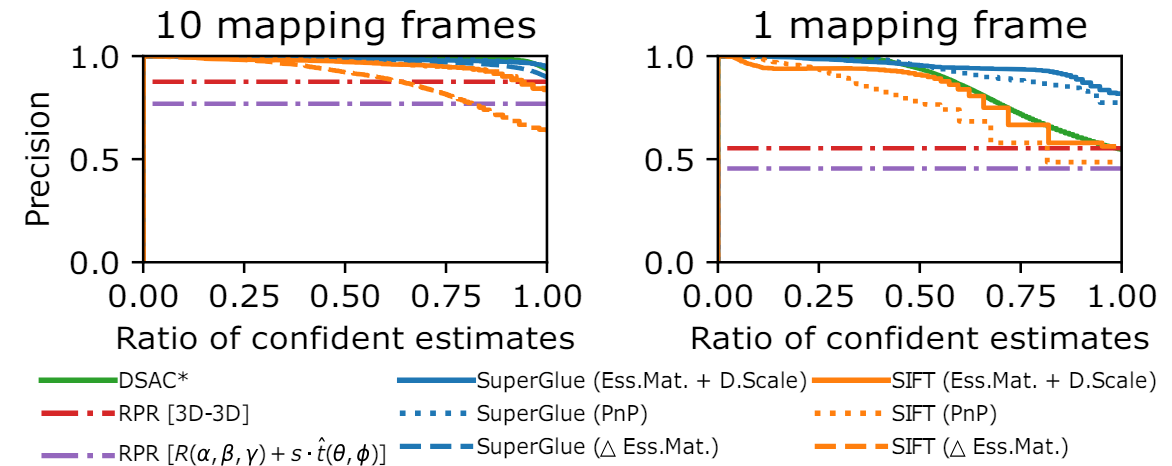
\includegraphics[scale=0.8]{pics/Proposal/partial_7scene.png}
  \caption[Hiệu quả của các mô hình khi giới hạn ảnh tham khảo]{Hiệu quả của những mô hình khi tập 7Scenes chỉ có 10/1 ảnh tham khảo, đánh giá về độ chính xác và về số ảnh có sai số phản chiếu dưới ngưỡng.}
\end{figure}

Để có thể phản ánh một môi trường thực tế, nơi mà ảnh tham khảo truy xuất được cách xa một khoảng đáng kể so với ảnh truy vấn, $K$ ảnh tham khảo mang nhiều thông tin nhất sẽ được chọn làm đại diện qua giải thuật gom cụm K-means.

Với việc so sánh độ chính xác ở hai kịch bản, ngưỡng chấp nhận về độ chính xác sẽ là $VCRE<10\%$ của đường chéo ảnh(80px). Khi ngưỡng tin cậy được hạ thấp, điều này làm cho tỷ lệ số dự đoán đáng tin cậy tăng lên. Điều này làm độ chính xác giảm dần, do chứa những trường hợp có độ tin cậy không đủ cao. Trong trường hợp này, những mô hình 2D-2D, đặc biệt là mô hình sử dụng SuperGlue, có kết quả tốt hơn so với những mô hình còn lại. Điều này thể hiện rõ nhất trong khoảng $0.5~1.0$. Ngoài ra, mô hình 2D-2D có thể tính ra vị trí và góc quay của hơn 50\% ảnh với VCRE < 40px.

Mô hình DSAC* vẫn có kết quả tốt nhất trong các mô hình. Tuy nhiên, phương pháp này lại quá phụ thuộc vào tập dữ liệu. Trong khi đó, những mô hình khác được huấn luyện trên tập ScanNet vẫn có kết quả tốt trên tập 7Scenes. Phương pháp sử dụng phép đạc tam giác cũng có kết quả cạnh tranh, tuy nhiên lại không thể hoạt động chỉ với một ảnh tham khảo. Những phương pháp ghép cặp đặc trưng + tính toán độ sâu có khả năng khái quát hóa tốt hơn những phương pháp RPR, có thể thấy ở hiệu quả tương đối thấp hơn của những phương pháp hồi quy vị trí tương đối.
\newpage
\textbf{Tập dữ liệu Niantic \cite{arnold2022mapfree}}

\begin{figure}[H]
  \centering
  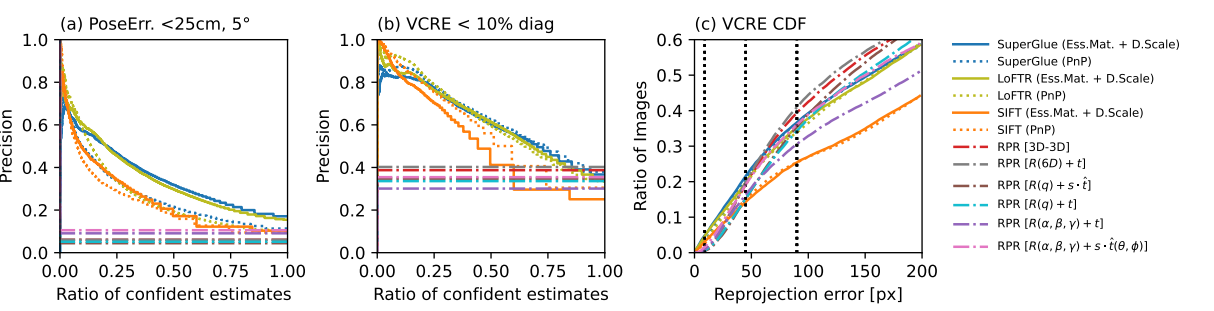
\includegraphics[scale=0.75]{pics/Proposal/all_niantic.png}
  \caption{Hiệu quả của các mô hình trên tập dữ liệu Niantic, xác định theo độ chính xác và số ảnh có sai số phản chiếu dưới ngưỡng}
\end{figure}

Qua kết quả thu được, tập dữ liệu Niantic có độ khó cao hơn đáng kể so với tập dữ liệu 7Scenes với mọi phương pháp. Điều này có thể thấy được rõ ràng từ kết quả của các mô hình. Trong tập dữ liệu Niantic, những phương pháp 2D-2D tiếp tục có kết quả tốt. Tuy nhiên, ở những ngưỡng VCRE rộng hơn, những phương pháp RPR lại có kết quả tốt hơn. Điều này có thể giải thích được qua việc khi số cặp đặc trưng tương quan là không đủ chất lượng, độ lệch đơn vị vị trí được sinh ra có thể có sai số rất lớn so với thực tế. Vậy nên, những phương pháp RPR sẽ cho ra kết quả tốt khi ngưỡng chính xác rộng, nhưng lại có kết quả không tốt khi cần độ chính xác cao. Ngoài ra, những phương pháp RPR cũng không thể cung cấp độ tin cậy cho dự đoán của mô hình: không thể loại bỏ những dự đoán có khả năng sai cao.
